\documentclass[twoside]{book}

% Packages required by doxygen
\usepackage{calc}
\usepackage{doxygen}
\usepackage{graphicx}
\usepackage[utf8]{inputenc}
\usepackage{makeidx}
\usepackage{multicol}
\usepackage{multirow}
\usepackage{textcomp}
\usepackage[table]{xcolor}

% Font selection
\usepackage[T1]{fontenc}
\usepackage{mathptmx}
\usepackage[scaled=.90]{helvet}
\usepackage{courier}
\usepackage{amssymb}
\usepackage{sectsty}
\renewcommand{\familydefault}{\sfdefault}
\allsectionsfont{%
  \fontseries{bc}\selectfont%
  \color{darkgray}%
}
\renewcommand{\DoxyLabelFont}{%
  \fontseries{bc}\selectfont%
  \color{darkgray}%
}

% Page & text layout
\usepackage{geometry}
\geometry{%
  a4paper,%
  top=2.5cm,%
  bottom=2.5cm,%
  left=2.5cm,%
  right=2.5cm%
}
\tolerance=750
\hfuzz=15pt
\hbadness=750
\setlength{\emergencystretch}{15pt}
\setlength{\parindent}{0cm}
\setlength{\parskip}{0.2cm}
\makeatletter
\renewcommand{\paragraph}{%
  \@startsection{paragraph}{4}{0ex}{-1.0ex}{1.0ex}{%
    \normalfont\normalsize\bfseries\SS@parafont%
  }%
}
\renewcommand{\subparagraph}{%
  \@startsection{subparagraph}{5}{0ex}{-1.0ex}{1.0ex}{%
    \normalfont\normalsize\bfseries\SS@subparafont%
  }%
}
\makeatother

% Headers & footers
\usepackage{fancyhdr}
\pagestyle{fancyplain}
\fancyhead[LE]{\fancyplain{}{\bfseries\thepage}}
\fancyhead[CE]{\fancyplain{}{}}
\fancyhead[RE]{\fancyplain{}{\bfseries\leftmark}}
\fancyhead[LO]{\fancyplain{}{\bfseries\rightmark}}
\fancyhead[CO]{\fancyplain{}{}}
\fancyhead[RO]{\fancyplain{}{\bfseries\thepage}}
\fancyfoot[LE]{\fancyplain{}{}}
\fancyfoot[CE]{\fancyplain{}{}}
\fancyfoot[RE]{\fancyplain{}{\bfseries\scriptsize Generated on Fri Mar 14 2014 04\-:05\-:34 for Predictive Coding Toolbox by Doxygen }}
\fancyfoot[LO]{\fancyplain{}{\bfseries\scriptsize Generated on Fri Mar 14 2014 04\-:05\-:34 for Predictive Coding Toolbox by Doxygen }}
\fancyfoot[CO]{\fancyplain{}{}}
\fancyfoot[RO]{\fancyplain{}{}}
\renewcommand{\footrulewidth}{0.4pt}
\renewcommand{\chaptermark}[1]{%
  \markboth{#1}{}%
}
\renewcommand{\sectionmark}[1]{%
  \markright{\thesection\ #1}%
}

% Indices & bibliography
\usepackage{natbib}
\usepackage[titles]{tocloft}
\setcounter{tocdepth}{3}
\setcounter{secnumdepth}{5}
\makeindex

% Hyperlinks (required, but should be loaded last)
\usepackage{ifpdf}
\ifpdf
  \usepackage[pdftex,pagebackref=true]{hyperref}
\else
  \usepackage[ps2pdf,pagebackref=true]{hyperref}
\fi
\hypersetup{%
  colorlinks=true,%
  linkcolor=blue,%
  citecolor=blue,%
  unicode%
}

% Custom commands
\newcommand{\clearemptydoublepage}{%
  \newpage{\pagestyle{empty}\cleardoublepage}%
}


%===== C O N T E N T S =====

\begin{document}

% Titlepage & ToC
\hypersetup{pageanchor=false}
\pagenumbering{roman}
\begin{titlepage}
\vspace*{7cm}
\begin{center}%
{\Large Predictive Coding Toolbox }\\
\vspace*{1cm}
{\large Generated by Doxygen 1.8.5}\\
\vspace*{0.5cm}
{\small Fri Mar 14 2014 04:05:34}\\
\end{center}
\end{titlepage}
\clearemptydoublepage
\tableofcontents
\clearemptydoublepage
\pagenumbering{arabic}
\hypersetup{pageanchor=true}

%--- Begin generated contents ---
\chapter{Main Page}
\label{index}\hypertarget{index}{}The Predictive Coding Toolbox, or P\-C\-T for short, is a set of tools that is designed to help with research on the Predictive Coding framework.\hypertarget{index_sec_pages}{}\section{Pages}\label{index_sec_pages}
\begin{DoxyItemize}
\item the \hyperlink{manual}{User Manual} \item A \hyperlink{group__tools}{list} of available tools and their uses \item Creating \hyperlink{query}{queries} for inference \item Specifying Predictive Coding Hierarchies and performing \hyperlink{query}{inference} on them\end{DoxyItemize}
\hypertarget{index_sec_license}{}\section{License}\label{index_sec_license}
This toolbox uses the \href{http://genie.sis.pitt.edu/}{\tt S\-M\-I\-L\-E library}, which is made available \char`\"{}free of charge for any use\char`\"{} by the Decision Systems Laboratory of the University of Pittsburgh.

This toolbox itself is provided under the M\-I\-T license, reproduced below.

Copyright (c) 2014 Dennis Merkus

Permission is hereby granted, free of charge, to any person obtaining a copy of this software and associated documentation files (the \char`\"{}\-Software\char`\"{}), to deal in the Software without restriction, including without limitation the rights to use, copy, modify, merge, publish, distribute, sublicense, and/or sell copies of the Software, and to permit persons to whom the Software is furnished to do so, subject to the following conditions\-:

The above copyright notice and this permission notice shall be included in all copies or substantial portions of the Software.

T\-H\-E S\-O\-F\-T\-W\-A\-R\-E I\-S P\-R\-O\-V\-I\-D\-E\-D \char`\"{}\-A\-S I\-S\char`\"{}, W\-I\-T\-H\-O\-U\-T W\-A\-R\-R\-A\-N\-T\-Y O\-F A\-N\-Y K\-I\-N\-D, E\-X\-P\-R\-E\-S\-S O\-R I\-M\-P\-L\-I\-E\-D, I\-N\-C\-L\-U\-D\-I\-N\-G B\-U\-T N\-O\-T L\-I\-M\-I\-T\-E\-D T\-O T\-H\-E W\-A\-R\-R\-A\-N\-T\-I\-E\-S O\-F M\-E\-R\-C\-H\-A\-N\-T\-A\-B\-I\-L\-I\-T\-Y, F\-I\-T\-N\-E\-S\-S F\-O\-R A P\-A\-R\-T\-I\-C\-U\-L\-A\-R P\-U\-R\-P\-O\-S\-E A\-N\-D N\-O\-N\-I\-N\-F\-R\-I\-N\-G\-E\-M\-E\-N\-T. I\-N N\-O E\-V\-E\-N\-T S\-H\-A\-L\-L T\-H\-E A\-U\-T\-H\-O\-R\-S O\-R C\-O\-P\-Y\-R\-I\-G\-H\-T H\-O\-L\-D\-E\-R\-S B\-E L\-I\-A\-B\-L\-E F\-O\-R A\-N\-Y C\-L\-A\-I\-M, D\-A\-M\-A\-G\-E\-S O\-R O\-T\-H\-E\-R L\-I\-A\-B\-I\-L\-I\-T\-Y, W\-H\-E\-T\-H\-E\-R I\-N A\-N A\-C\-T\-I\-O\-N O\-F C\-O\-N\-T\-R\-A\-C\-T, T\-O\-R\-T O\-R O\-T\-H\-E\-R\-W\-I\-S\-E, A\-R\-I\-S\-I\-N\-G F\-R\-O\-M, O\-U\-T O\-F O\-R I\-N C\-O\-N\-N\-E\-C\-T\-I\-O\-N W\-I\-T\-H T\-H\-E S\-O\-F\-T\-W\-A\-R\-E O\-R T\-H\-E U\-S\-E O\-R O\-T\-H\-E\-R D\-E\-A\-L\-I\-N\-G\-S I\-N T\-H\-E S\-O\-F\-T\-W\-A\-R\-E. 
\chapter{Developer Manual}
\label{developer}
\hypertarget{developer}{}
\hypertarget{developer_dev_tool}{}\section{Adding a New Tool}\label{developer_dev_tool}

\chapter{Querying Probabilities}
\label{query}
\hypertarget{query}{}
The (simplified) B\-N\-F grammar for the queries is as follows\-:

\begin{DoxyVerb}* Query       := 'P(' Body ')'
* Body        := Terms '|' Terms | Terms
* Terms       := Term ',' Terms | Term
* Term        := Variable '=' Value | Variable
*
* Variable    := {any valid node name}
* Value       := {any valid value identifier}
* \end{DoxyVerb}
 
\chapter{User Manual}
\label{manual}
\hypertarget{manual}{}
\hypertarget{manual_manual_intro}{}\section{Introduction}\label{manual_manual_intro}
\hypertarget{manual_manual_flow}{}\section{Information Flow}\label{manual_manual_flow}
\hypertarget{manual_manual_tools}{}\section{Tools}\label{manual_manual_tools}

\chapter{Module Index}
\section{Modules}
Here is a list of all modules\-:\begin{DoxyCompactList}
\item \contentsline{section}{Tools in the Predictive Coding Toolbox}{\pageref{group__tools}}{}
\end{DoxyCompactList}

\chapter{Hierarchical Index}
\section{Class Hierarchy}
This inheritance list is sorted roughly, but not completely, alphabetically\-:\begin{DoxyCompactList}
\item \contentsline{section}{pct\-:\-:Bayesian\-Network}{\pageref{classpct_1_1_bayesian_network}}{}
\begin{DoxyCompactList}
\item \contentsline{section}{pct\-:\-:S\-M\-I\-L\-E\-Bayesian\-Network}{\pageref{classpct_1_1_s_m_i_l_e_bayesian_network}}{}
\end{DoxyCompactList}
\item \contentsline{section}{pct\-:\-:Info}{\pageref{classpct_1_1_info}}{}
\item \contentsline{section}{pct\-:\-:Info\-Set}{\pageref{classpct_1_1_info_set}}{}
\item \contentsline{section}{pct\-:\-:Module}{\pageref{classpct_1_1_module}}{}
\begin{DoxyCompactList}
\item \contentsline{section}{pct\-:\-:File\-Input\-Module}{\pageref{classpct_1_1_file_input_module}}{}
\end{DoxyCompactList}
\item \contentsline{section}{pct\-:\-:Parser}{\pageref{classpct_1_1_parser}}{}
\item \contentsline{section}{pct\-:\-:pc\-:\-:P\-C\-Hierarchy}{\pageref{classpct_1_1pc_1_1_p_c_hierarchy}}{}
\item \contentsline{section}{pct\-:\-:pc\-:\-:P\-C\-Network}{\pageref{classpct_1_1pc_1_1_p_c_network}}{}
\item \contentsline{section}{pct\-:\-:Predictive\-Coding\-Toolbox}{\pageref{classpct_1_1_predictive_coding_toolbox}}{}
\item \contentsline{section}{pct\-:\-:Query}{\pageref{classpct_1_1_query}}{}
\item \contentsline{section}{Test}{\pageref{class_test}}{}
\item \contentsline{section}{pct\-:\-:Token}{\pageref{classpct_1_1_token}}{}
\item \contentsline{section}{pct\-:\-:Tool}{\pageref{classpct_1_1_tool}}{}
\begin{DoxyCompactList}
\item \contentsline{section}{pct\-:\-:Analysis\-Tool}{\pageref{classpct_1_1_analysis_tool}}{}
\item \contentsline{section}{pct\-:\-:Inference\-Tool}{\pageref{classpct_1_1_inference_tool}}{}
\end{DoxyCompactList}
\item \contentsline{section}{pct\-:\-:Variable}{\pageref{classpct_1_1_variable}}{}
\end{DoxyCompactList}

\chapter{Class Index}
\section{Class List}
Here are the classes, structs, unions and interfaces with brief descriptions\-:\begin{DoxyCompactList}
\item\contentsline{section}{\hyperlink{classpct_1_1_analysis_tool}{pct\-::\-Analysis\-Tool} }{\pageref{classpct_1_1_analysis_tool}}{}
\item\contentsline{section}{\hyperlink{classpct_1_1_bayesian_network}{pct\-::\-Bayesian\-Network} }{\pageref{classpct_1_1_bayesian_network}}{}
\item\contentsline{section}{\hyperlink{classpct_1_1_file_input_module}{pct\-::\-File\-Input\-Module} }{\pageref{classpct_1_1_file_input_module}}{}
\item\contentsline{section}{\hyperlink{classpct_1_1_inference_tool}{pct\-::\-Inference\-Tool} }{\pageref{classpct_1_1_inference_tool}}{}
\item\contentsline{section}{\hyperlink{classpct_1_1_info}{pct\-::\-Info} }{\pageref{classpct_1_1_info}}{}
\item\contentsline{section}{\hyperlink{classpct_1_1_info_set}{pct\-::\-Info\-Set} \\*Provides labeled information }{\pageref{classpct_1_1_info_set}}{}
\item\contentsline{section}{\hyperlink{classpct_1_1_module}{pct\-::\-Module} }{\pageref{classpct_1_1_module}}{}
\item\contentsline{section}{\hyperlink{classpct_1_1_parser}{pct\-::\-Parser} \\*Implements the probability parser for the specified grammar }{\pageref{classpct_1_1_parser}}{}
\item\contentsline{section}{\hyperlink{classpct_1_1pc_1_1_p_c_hierarchy}{pct\-::pc\-::\-P\-C\-Hierarchy} }{\pageref{classpct_1_1pc_1_1_p_c_hierarchy}}{}
\item\contentsline{section}{\hyperlink{classpct_1_1pc_1_1_p_c_network}{pct\-::pc\-::\-P\-C\-Network} \\*A single network within the Predictive Coding framework }{\pageref{classpct_1_1pc_1_1_p_c_network}}{}
\item\contentsline{section}{\hyperlink{classpct_1_1_predictive_coding_toolbox}{pct\-::\-Predictive\-Coding\-Toolbox} \\*Main class for the Predictive Coding Toolbox }{\pageref{classpct_1_1_predictive_coding_toolbox}}{}
\item\contentsline{section}{\hyperlink{classpct_1_1_query}{pct\-::\-Query} }{\pageref{classpct_1_1_query}}{}
\item\contentsline{section}{\hyperlink{classpct_1_1_s_m_i_l_e_bayesian_network}{pct\-::\-S\-M\-I\-L\-E\-Bayesian\-Network} }{\pageref{classpct_1_1_s_m_i_l_e_bayesian_network}}{}
\item\contentsline{section}{\hyperlink{class_test}{Test} }{\pageref{class_test}}{}
\item\contentsline{section}{\hyperlink{classpct_1_1_token}{pct\-::\-Token} }{\pageref{classpct_1_1_token}}{}
\item\contentsline{section}{\hyperlink{classpct_1_1_tool}{pct\-::\-Tool} }{\pageref{classpct_1_1_tool}}{}
\item\contentsline{section}{\hyperlink{classpct_1_1_variable}{pct\-::\-Variable} }{\pageref{classpct_1_1_variable}}{}
\end{DoxyCompactList}

\chapter{File Index}
\section{File List}
Here is a list of all documented files with brief descriptions\-:\begin{DoxyCompactList}
\item\contentsline{section}{{\bfseries analysistool.\-hpp} }{\pageref{analysistool_8hpp}}{}
\item\contentsline{section}{{\bfseries fileinputmodule.\-hpp} }{\pageref{fileinputmodule_8hpp}}{}
\item\contentsline{section}{{\bfseries inferencetool.\-hpp} }{\pageref{inferencetool_8hpp}}{}
\item\contentsline{section}{{\bfseries info.\-hpp} }{\pageref{info_8hpp}}{}
\item\contentsline{section}{{\bfseries infoset.\-hpp} }{\pageref{infoset_8hpp}}{}
\item\contentsline{section}{{\bfseries module.\-hpp} }{\pageref{module_8hpp}}{}
\item\contentsline{section}{\hyperlink{network_8hpp}{network.\-hpp} }{\pageref{network_8hpp}}{}
\item\contentsline{section}{{\bfseries parser.\-hpp} }{\pageref{parser_8hpp}}{}
\item\contentsline{section}{{\bfseries pchierarchy.\-hpp} }{\pageref{pchierarchy_8hpp}}{}
\item\contentsline{section}{{\bfseries pcnetwork.\-hpp} }{\pageref{pcnetwork_8hpp}}{}
\item\contentsline{section}{\hyperlink{pct_8hpp}{pct.\-hpp} }{\pageref{pct_8hpp}}{}
\item\contentsline{section}{{\bfseries query.\-hpp} }{\pageref{query_8hpp}}{}
\item\contentsline{section}{{\bfseries test.\-hpp} }{\pageref{test_8hpp}}{}
\item\contentsline{section}{{\bfseries token.\-hpp} }{\pageref{token_8hpp}}{}
\item\contentsline{section}{{\bfseries tool.\-hpp} }{\pageref{tool_8hpp}}{}
\item\contentsline{section}{{\bfseries variable.\-hpp} }{\pageref{variable_8hpp}}{}
\end{DoxyCompactList}

\chapter{Module Documentation}
\hypertarget{group__tools}{\section{Tools in the Predictive Coding Toolbox}
\label{group__tools}\index{Tools in the Predictive Coding Toolbox@{Tools in the Predictive Coding Toolbox}}
}


This is a test.  


This is a test. This is another test.
\chapter{Class Documentation}
\hypertarget{classpct_1_1_analysis_tool}{\section{pct\-:\-:Analysis\-Tool Class Reference}
\label{classpct_1_1_analysis_tool}\index{pct\-::\-Analysis\-Tool@{pct\-::\-Analysis\-Tool}}
}


Inheritance diagram for pct\-:\-:Analysis\-Tool\-:\nopagebreak
\begin{figure}[H]
\begin{center}
\leavevmode
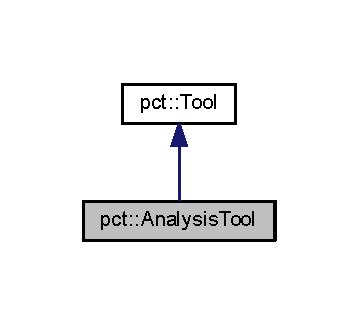
\includegraphics[width=172pt]{classpct_1_1_analysis_tool__inherit__graph}
\end{center}
\end{figure}


Collaboration diagram for pct\-:\-:Analysis\-Tool\-:\nopagebreak
\begin{figure}[H]
\begin{center}
\leavevmode
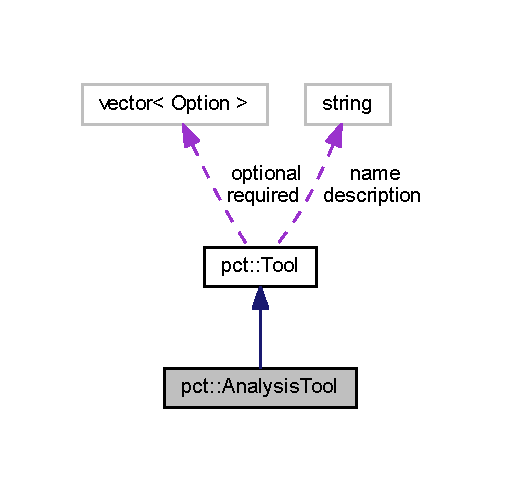
\includegraphics[width=243pt]{classpct_1_1_analysis_tool__coll__graph}
\end{center}
\end{figure}
\subsection*{Public Member Functions}
\begin{DoxyCompactItemize}
\item 
\hypertarget{classpct_1_1_analysis_tool_a468222469d5be7ff5d2fdc39730449f2}{virtual \hyperlink{classpct_1_1_info_set}{Info\-Set} {\bfseries run} (\hyperlink{classpct_1_1_info_set}{Info\-Set} options)}\label{classpct_1_1_analysis_tool_a468222469d5be7ff5d2fdc39730449f2}

\item 
\hypertarget{classpct_1_1_analysis_tool_ac4439367354e4b230b0b206ee9d2a331}{virtual string {\bfseries get\-Option\-Help} (string name)}\label{classpct_1_1_analysis_tool_ac4439367354e4b230b0b206ee9d2a331}

\end{DoxyCompactItemize}
\subsection*{Additional Inherited Members}


The documentation for this class was generated from the following files\-:\begin{DoxyCompactItemize}
\item 
analysistool.\-hpp\item 
analysistool.\-cpp\end{DoxyCompactItemize}

\hypertarget{classpct_1_1_bayesian_network}{\section{pct\-:\-:Bayesian\-Network Class Reference}
\label{classpct_1_1_bayesian_network}\index{pct\-::\-Bayesian\-Network@{pct\-::\-Bayesian\-Network}}
}


Inheritance diagram for pct\-:\-:Bayesian\-Network\-:\nopagebreak
\begin{figure}[H]
\begin{center}
\leavevmode
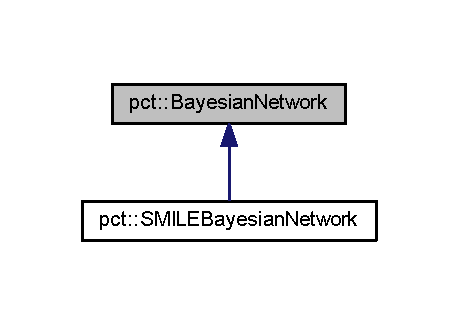
\includegraphics[width=220pt]{classpct_1_1_bayesian_network__inherit__graph}
\end{center}
\end{figure}
\subsection*{Public Member Functions}
\begin{DoxyCompactItemize}
\item 
\hypertarget{classpct_1_1_bayesian_network_a25de1a5a824d2d01c5c043c0a213e04a}{virtual void {\bfseries add\-Node} (string name, vector$<$ string $>$ values)=0}\label{classpct_1_1_bayesian_network_a25de1a5a824d2d01c5c043c0a213e04a}

\item 
\hypertarget{classpct_1_1_bayesian_network_a656d12f66b031e4c85461e05df2e58e5}{virtual void {\bfseries add\-Dependency} (string from, string to)=0}\label{classpct_1_1_bayesian_network_a656d12f66b031e4c85461e05df2e58e5}

\item 
\hypertarget{classpct_1_1_bayesian_network_a66214e737a33c21e4fda5849d9eb771a}{virtual void {\bfseries write\-File} (string name, File\-Format format=D\-S\-L)=0}\label{classpct_1_1_bayesian_network_a66214e737a33c21e4fda5849d9eb771a}

\item 
\hypertarget{classpct_1_1_bayesian_network_accc06218f488d68a73b1f9e1144b1d18}{virtual void {\bfseries set\-Algorithm} (string name)=0}\label{classpct_1_1_bayesian_network_accc06218f488d68a73b1f9e1144b1d18}

\item 
\hypertarget{classpct_1_1_bayesian_network_a5f36ad6abc527a1aba7ccecb8b6d4300}{virtual void {\bfseries update} ()=0}\label{classpct_1_1_bayesian_network_a5f36ad6abc527a1aba7ccecb8b6d4300}

\item 
\hypertarget{classpct_1_1_bayesian_network_ae382925bdc9910878a0f636ed85a9b65}{virtual void {\bfseries calculate\-Distribution} (\hyperlink{classpct_1_1_query}{Query} query)=0}\label{classpct_1_1_bayesian_network_ae382925bdc9910878a0f636ed85a9b65}

\end{DoxyCompactItemize}
\subsection*{Static Public Member Functions}
\begin{DoxyCompactItemize}
\item 
\hypertarget{classpct_1_1_bayesian_network_a20a0fb1dd2050c25945decda2ae772bb}{static string {\bfseries display\-Possible\-Algorithms} ()}\label{classpct_1_1_bayesian_network_a20a0fb1dd2050c25945decda2ae772bb}

\end{DoxyCompactItemize}


The documentation for this class was generated from the following files\-:\begin{DoxyCompactItemize}
\item 
\hyperlink{network_8hpp}{network.\-hpp}\item 
network.\-cpp\end{DoxyCompactItemize}

\hypertarget{classpct_1_1_file_input_module}{\section{pct\-:\-:File\-Input\-Module Class Reference}
\label{classpct_1_1_file_input_module}\index{pct\-::\-File\-Input\-Module@{pct\-::\-File\-Input\-Module}}
}


Inheritance diagram for pct\-:\-:File\-Input\-Module\-:\nopagebreak
\begin{figure}[H]
\begin{center}
\leavevmode
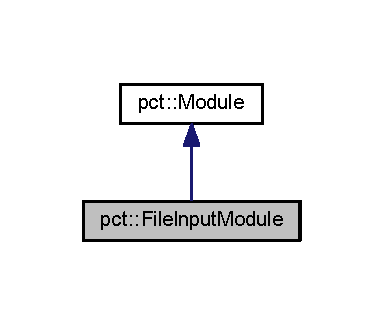
\includegraphics[width=184pt]{classpct_1_1_file_input_module__inherit__graph}
\end{center}
\end{figure}


Collaboration diagram for pct\-:\-:File\-Input\-Module\-:\nopagebreak
\begin{figure}[H]
\begin{center}
\leavevmode
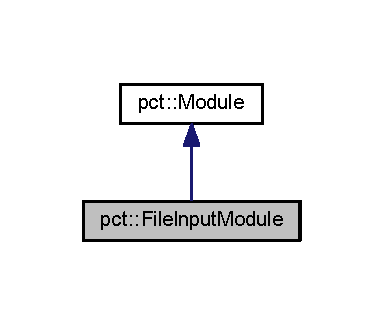
\includegraphics[width=184pt]{classpct_1_1_file_input_module__coll__graph}
\end{center}
\end{figure}
\subsection*{Static Public Member Functions}
\begin{DoxyCompactItemize}
\item 
\hypertarget{classpct_1_1_file_input_module_ac8f804700eb906655dfdf550c1ba36c6}{static \hyperlink{classpct_1_1_s_m_i_l_e_bayesian_network}{S\-M\-I\-L\-E\-Bayesian\-Network} {\bfseries load} (string name)}\label{classpct_1_1_file_input_module_ac8f804700eb906655dfdf550c1ba36c6}

\end{DoxyCompactItemize}


The documentation for this class was generated from the following files\-:\begin{DoxyCompactItemize}
\item 
fileinputmodule.\-hpp\item 
fileinputmodule.\-cpp\end{DoxyCompactItemize}

\hypertarget{classpct_1_1_inference_tool}{\section{pct\-:\-:Inference\-Tool Class Reference}
\label{classpct_1_1_inference_tool}\index{pct\-::\-Inference\-Tool@{pct\-::\-Inference\-Tool}}
}


Inheritance diagram for pct\-:\-:Inference\-Tool\-:\nopagebreak
\begin{figure}[H]
\begin{center}
\leavevmode
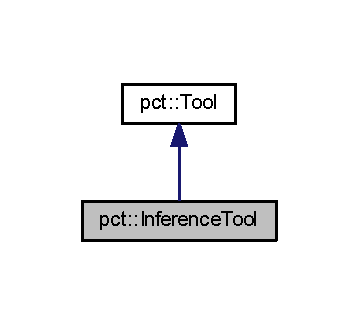
\includegraphics[width=172pt]{classpct_1_1_inference_tool__inherit__graph}
\end{center}
\end{figure}


Collaboration diagram for pct\-:\-:Inference\-Tool\-:\nopagebreak
\begin{figure}[H]
\begin{center}
\leavevmode
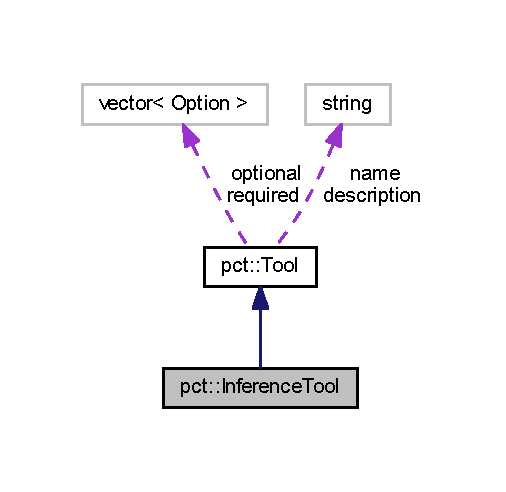
\includegraphics[width=243pt]{classpct_1_1_inference_tool__coll__graph}
\end{center}
\end{figure}
\subsection*{Public Member Functions}
\begin{DoxyCompactItemize}
\item 
\hypertarget{classpct_1_1_inference_tool_ad0ed8739f52c7a8914a9fd1939b35e49}{virtual \hyperlink{classpct_1_1_info_set}{Info\-Set} {\bfseries run} (\hyperlink{classpct_1_1_info_set}{Info\-Set} options)}\label{classpct_1_1_inference_tool_ad0ed8739f52c7a8914a9fd1939b35e49}

\item 
\hypertarget{classpct_1_1_inference_tool_a6fe6b41458fd550575611156491ea203}{virtual string {\bfseries get\-Option\-Help} (string name)}\label{classpct_1_1_inference_tool_a6fe6b41458fd550575611156491ea203}

\end{DoxyCompactItemize}
\subsection*{Additional Inherited Members}


The documentation for this class was generated from the following files\-:\begin{DoxyCompactItemize}
\item 
inferencetool.\-hpp\item 
inferencetool.\-cpp\end{DoxyCompactItemize}

\hypertarget{classpct_1_1_info}{\section{pct\-:\-:Info Class Reference}
\label{classpct_1_1_info}\index{pct\-::\-Info@{pct\-::\-Info}}
}
\subsection*{Public Types}
\begin{DoxyCompactItemize}
\item 
enum {\bfseries Type} \{ {\bfseries Integer}, 
{\bfseries Double}, 
{\bfseries String}
 \}
\end{DoxyCompactItemize}
\subsection*{Public Member Functions}
\begin{DoxyCompactItemize}
\item 
\hypertarget{classpct_1_1_info_a243ba2b48910ca6f8be684d05cf4a069}{{\bfseries Info} (string name, string value)}\label{classpct_1_1_info_a243ba2b48910ca6f8be684d05cf4a069}

\item 
\hypertarget{classpct_1_1_info_abf88a6e4bdc20e266b71b55d1c940c86}{{\bfseries Info} (string name, int value)}\label{classpct_1_1_info_abf88a6e4bdc20e266b71b55d1c940c86}

\item 
\hypertarget{classpct_1_1_info_a9bbe668631758b5852ae82c06483fc0c}{{\bfseries Info} (string name, double value)}\label{classpct_1_1_info_a9bbe668631758b5852ae82c06483fc0c}

\item 
\hypertarget{classpct_1_1_info_a4dacb0c9e8230aa06416495db023a5b6}{string {\bfseries get\-Name} ()}\label{classpct_1_1_info_a4dacb0c9e8230aa06416495db023a5b6}

\item 
\hypertarget{classpct_1_1_info_a78274768236c7e9e00c396948c54dcfa}{Type {\bfseries get\-Type} ()}\label{classpct_1_1_info_a78274768236c7e9e00c396948c54dcfa}

\item 
\hypertarget{classpct_1_1_info_abff5f374352edf4fbd6eafacbfa0c8a8}{int {\bfseries get\-Int\-Value} ()}\label{classpct_1_1_info_abff5f374352edf4fbd6eafacbfa0c8a8}

\item 
\hypertarget{classpct_1_1_info_a7d139540adcb8d78c5a353416074d680}{double {\bfseries get\-Double\-Value} ()}\label{classpct_1_1_info_a7d139540adcb8d78c5a353416074d680}

\item 
\hypertarget{classpct_1_1_info_a5a5de77be24d0f0857fca0277951943b}{string {\bfseries get\-String\-Value} ()}\label{classpct_1_1_info_a5a5de77be24d0f0857fca0277951943b}

\end{DoxyCompactItemize}


The documentation for this class was generated from the following files\-:\begin{DoxyCompactItemize}
\item 
info.\-hpp\item 
info.\-cpp\end{DoxyCompactItemize}

\hypertarget{classpct_1_1_info_set}{\section{pct\-:\-:Info\-Set Class Reference}
\label{classpct_1_1_info_set}\index{pct\-::\-Info\-Set@{pct\-::\-Info\-Set}}
}


Provides labeled information.  




{\ttfamily \#include $<$infoset.\-hpp$>$}

\subsection*{Public Member Functions}
\begin{DoxyCompactItemize}
\item 
\hypertarget{classpct_1_1_info_set_af60815077cca5f9de8a2fa5fb5424163}{\hyperlink{classpct_1_1_info_set_af60815077cca5f9de8a2fa5fb5424163}{Info\-Set} ()}\label{classpct_1_1_info_set_af60815077cca5f9de8a2fa5fb5424163}

\begin{DoxyCompactList}\small\item\em Creates a container without any information. \end{DoxyCompactList}\item 
void \hyperlink{classpct_1_1_info_set_a6daa0aeffdacaca7b466e8a8c79b60b8}{add\-Info} (\hyperlink{classpct_1_1_info}{Info} info)
\begin{DoxyCompactList}\small\item\em Add one particular piece of information. \end{DoxyCompactList}\item 
\hypertarget{classpct_1_1_info_set_a1f438cef60c6905e6ecf658f35bc8067}{void \hyperlink{classpct_1_1_info_set_a1f438cef60c6905e6ecf658f35bc8067}{set\-Flag} (string name)}\label{classpct_1_1_info_set_a1f438cef60c6905e6ecf658f35bc8067}

\begin{DoxyCompactList}\small\item\em Sets the flag with the specified name. \end{DoxyCompactList}\item 
\hypertarget{classpct_1_1_info_set_ac89b9f99c5323af0eb2f70d59c64515b}{bool \hyperlink{classpct_1_1_info_set_ac89b9f99c5323af0eb2f70d59c64515b}{contains} (string name)}\label{classpct_1_1_info_set_ac89b9f99c5323af0eb2f70d59c64515b}

\begin{DoxyCompactList}\small\item\em Determine whether information with the specified name is already present. \end{DoxyCompactList}\item 
\hypertarget{classpct_1_1_info_set_a10de2ed5cd357b1fe4c9b2cedd2f7622}{bool \hyperlink{classpct_1_1_info_set_a10de2ed5cd357b1fe4c9b2cedd2f7622}{is\-Set} (string name)}\label{classpct_1_1_info_set_a10de2ed5cd357b1fe4c9b2cedd2f7622}

\begin{DoxyCompactList}\small\item\em Determine whether the flag with the specified name is set. \end{DoxyCompactList}\item 
\hypertarget{classpct_1_1_info_set_a762e6aa4218fb0743bc6f3b25b1681d9}{\hyperlink{classpct_1_1_info}{Info} \hyperlink{classpct_1_1_info_set_a762e6aa4218fb0743bc6f3b25b1681d9}{get\-Info} (string name)}\label{classpct_1_1_info_set_a762e6aa4218fb0743bc6f3b25b1681d9}

\begin{DoxyCompactList}\small\item\em Get the piece of information with the specified name. \end{DoxyCompactList}\item 
\hypertarget{classpct_1_1_info_set_afb54aabd6af682f26d8f3288b15d5f23}{string \hyperlink{classpct_1_1_info_set_afb54aabd6af682f26d8f3288b15d5f23}{display} ()}\label{classpct_1_1_info_set_afb54aabd6af682f26d8f3288b15d5f23}

\begin{DoxyCompactList}\small\item\em Create a visual representation of all the current information. \end{DoxyCompactList}\end{DoxyCompactItemize}


\subsection{Detailed Description}
Provides labeled information. 

Can be used both to specify parameters or to give results. 

\subsection{Member Function Documentation}
\hypertarget{classpct_1_1_info_set_a6daa0aeffdacaca7b466e8a8c79b60b8}{\index{pct\-::\-Info\-Set@{pct\-::\-Info\-Set}!add\-Info@{add\-Info}}
\index{add\-Info@{add\-Info}!pct::InfoSet@{pct\-::\-Info\-Set}}
\subsubsection[{add\-Info}]{\setlength{\rightskip}{0pt plus 5cm}void pct\-::\-Info\-Set\-::add\-Info (
\begin{DoxyParamCaption}
\item[{{\bf Info}}]{info}
\end{DoxyParamCaption}
)}}\label{classpct_1_1_info_set_a6daa0aeffdacaca7b466e8a8c79b60b8}


Add one particular piece of information. 

When there is a conflict with an already existing piece of information, nothing is altered. 

The documentation for this class was generated from the following files\-:\begin{DoxyCompactItemize}
\item 
infoset.\-hpp\item 
infoset.\-cpp\end{DoxyCompactItemize}

\hypertarget{classpct_1_1_module}{\section{pct\-:\-:Module Class Reference}
\label{classpct_1_1_module}\index{pct\-::\-Module@{pct\-::\-Module}}
}


Inheritance diagram for pct\-:\-:Module\-:\nopagebreak
\begin{figure}[H]
\begin{center}
\leavevmode
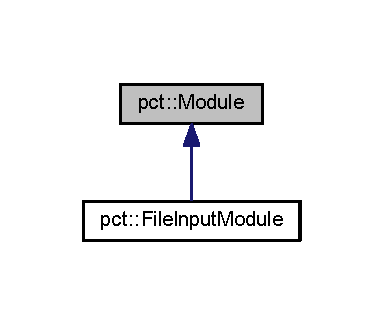
\includegraphics[width=184pt]{classpct_1_1_module__inherit__graph}
\end{center}
\end{figure}


The documentation for this class was generated from the following file\-:\begin{DoxyCompactItemize}
\item 
module.\-hpp\end{DoxyCompactItemize}

\hypertarget{classpct_1_1_parser}{\section{pct\-:\-:Parser Class Reference}
\label{classpct_1_1_parser}\index{pct\-::\-Parser@{pct\-::\-Parser}}
}


Implements the probability parser for the specified grammar.  




{\ttfamily \#include $<$parser.\-hpp$>$}

\subsection*{Public Member Functions}
\begin{DoxyCompactItemize}
\item 
\hyperlink{classpct_1_1_query}{Query} \hyperlink{classpct_1_1_parser_ab9168d205593af320ce89bb8ad8ff8a1}{parse} (string query)
\end{DoxyCompactItemize}


\subsection{Detailed Description}
Implements the probability parser for the specified grammar. 

\subsection{Member Function Documentation}
\hypertarget{classpct_1_1_parser_ab9168d205593af320ce89bb8ad8ff8a1}{\index{pct\-::\-Parser@{pct\-::\-Parser}!parse@{parse}}
\index{parse@{parse}!pct::Parser@{pct\-::\-Parser}}
\subsubsection[{parse}]{\setlength{\rightskip}{0pt plus 5cm}{\bf Query} pct\-::\-Parser\-::parse (
\begin{DoxyParamCaption}
\item[{string}]{query}
\end{DoxyParamCaption}
)}}\label{classpct_1_1_parser_ab9168d205593af320ce89bb8ad8ff8a1}
\begin{DoxySeeAlso}{See Also}
query 
\end{DoxySeeAlso}


The documentation for this class was generated from the following files\-:\begin{DoxyCompactItemize}
\item 
parser.\-hpp\item 
parser.\-cpp\end{DoxyCompactItemize}

\hypertarget{classpct_1_1pc_1_1_p_c_hierarchy}{\section{pct\-:\-:pc\-:\-:P\-C\-Hierarchy Class Reference}
\label{classpct_1_1pc_1_1_p_c_hierarchy}\index{pct\-::pc\-::\-P\-C\-Hierarchy@{pct\-::pc\-::\-P\-C\-Hierarchy}}
}
\subsection*{Public Member Functions}
\begin{DoxyCompactItemize}
\item 
\hypertarget{classpct_1_1pc_1_1_p_c_hierarchy_a541515028f67150ff45e37905a2ba24e}{void \hyperlink{classpct_1_1pc_1_1_p_c_hierarchy_a541515028f67150ff45e37905a2ba24e}{add\-Network} (\hyperlink{classpct_1_1pc_1_1_p_c_network}{P\-C\-Network} net)}\label{classpct_1_1pc_1_1_p_c_hierarchy_a541515028f67150ff45e37905a2ba24e}

\begin{DoxyCompactList}\small\item\em Adds a parentless network to the hierarchy. \end{DoxyCompactList}\item 
void \hyperlink{classpct_1_1pc_1_1_p_c_hierarchy_ac577e22bdf204af786b93242b3b826f6}{add\-Network} (\hyperlink{classpct_1_1pc_1_1_p_c_network}{P\-C\-Network} net, string parent, vector$<$ Link $>$ links)
\begin{DoxyCompactList}\small\item\em Connects a network to an existing network in the hierarchy. \end{DoxyCompactList}\item 
\hypertarget{classpct_1_1pc_1_1_p_c_hierarchy_aedb4c077d40897706f2bb789d7633de2}{void {\bfseries perform\-Inference} (\hyperlink{classpct_1_1_query}{Query} query)}\label{classpct_1_1pc_1_1_p_c_hierarchy_aedb4c077d40897706f2bb789d7633de2}

\end{DoxyCompactItemize}


\subsection{Member Function Documentation}
\hypertarget{classpct_1_1pc_1_1_p_c_hierarchy_ac577e22bdf204af786b93242b3b826f6}{\index{pct\-::pc\-::\-P\-C\-Hierarchy@{pct\-::pc\-::\-P\-C\-Hierarchy}!add\-Network@{add\-Network}}
\index{add\-Network@{add\-Network}!pct::pc::PCHierarchy@{pct\-::pc\-::\-P\-C\-Hierarchy}}
\subsubsection[{add\-Network}]{\setlength{\rightskip}{0pt plus 5cm}void pct\-::pc\-::\-P\-C\-Hierarchy\-::add\-Network (
\begin{DoxyParamCaption}
\item[{{\bf P\-C\-Network}}]{net, }
\item[{string}]{parent, }
\item[{vector$<$ Link $>$}]{links}
\end{DoxyParamCaption}
)}}\label{classpct_1_1pc_1_1_p_c_hierarchy_ac577e22bdf204af786b93242b3b826f6}


Connects a network to an existing network in the hierarchy. 

This checks if the networks can be linked with the provided information. To be able to link network A to parent P\-:

\begin{DoxyItemize}
\item P should have the same number of predictions as the number of hypotheses in A; \item the values of these predictions and hypotheses should be matched\end{DoxyItemize}
If these conditions are met, then the new network is linked to the parent in the hierarchy and the linked nodes are considered as one.


\begin{DoxyParams}{Parameters}
{\em parent} & name of the parent network to connect this to. \\
\hline
{\em links} & this specifies which of the parent network's prediction are linked to which of the hypotheses in the new network. \\
\hline
\end{DoxyParams}


The documentation for this class was generated from the following file\-:\begin{DoxyCompactItemize}
\item 
pchierarchy.\-hpp\end{DoxyCompactItemize}

\hypertarget{classpct_1_1pc_1_1_p_c_network}{\section{pct\-:\-:pc\-:\-:P\-C\-Network Class Reference}
\label{classpct_1_1pc_1_1_p_c_network}\index{pct\-::pc\-::\-P\-C\-Network@{pct\-::pc\-::\-P\-C\-Network}}
}


A single network within the Predictive Coding framework.  




{\ttfamily \#include $<$pcnetwork.\-hpp$>$}

\subsection*{Public Member Functions}
\begin{DoxyCompactItemize}
\item 
\hypertarget{classpct_1_1pc_1_1_p_c_network_aef107b91f7e34a32e764fc58d35498a5}{void {\bfseries set\-Hypothesis} (string name)}\label{classpct_1_1pc_1_1_p_c_network_aef107b91f7e34a32e764fc58d35498a5}

\item 
\hypertarget{classpct_1_1pc_1_1_p_c_network_ac4183907b89e5e4602da81ee622aa855}{void {\bfseries set\-Prediction} (string name)}\label{classpct_1_1pc_1_1_p_c_network_ac4183907b89e5e4602da81ee622aa855}

\item 
string \hyperlink{classpct_1_1pc_1_1_p_c_network_a73262d8c1da222a66e971823641459df}{get\-P\-C\-Name} ()
\begin{DoxyCompactList}\small\item\em Receive the name that this part of the network has. \end{DoxyCompactList}\end{DoxyCompactItemize}


\subsection{Detailed Description}
A single network within the Predictive Coding framework. 

This network specifies both hypothesis nodes and prediction nodes. 

\subsection{Member Function Documentation}
\hypertarget{classpct_1_1pc_1_1_p_c_network_a73262d8c1da222a66e971823641459df}{\index{pct\-::pc\-::\-P\-C\-Network@{pct\-::pc\-::\-P\-C\-Network}!get\-P\-C\-Name@{get\-P\-C\-Name}}
\index{get\-P\-C\-Name@{get\-P\-C\-Name}!pct::pc::PCNetwork@{pct\-::pc\-::\-P\-C\-Network}}
\subsubsection[{get\-P\-C\-Name}]{\setlength{\rightskip}{0pt plus 5cm}string pct\-::pc\-::\-P\-C\-Network\-::get\-P\-C\-Name (
\begin{DoxyParamCaption}
{}
\end{DoxyParamCaption}
)}}\label{classpct_1_1pc_1_1_p_c_network_a73262d8c1da222a66e971823641459df}


Receive the name that this part of the network has. 

Mostly used within hierarchies to specify connections. 

The documentation for this class was generated from the following file\-:\begin{DoxyCompactItemize}
\item 
pcnetwork.\-hpp\end{DoxyCompactItemize}

\hypertarget{classpct_1_1_predictive_coding_toolbox}{\section{pct\-:\-:Predictive\-Coding\-Toolbox Class Reference}
\label{classpct_1_1_predictive_coding_toolbox}\index{pct\-::\-Predictive\-Coding\-Toolbox@{pct\-::\-Predictive\-Coding\-Toolbox}}
}


Main class for the Predictive Coding Toolbox.  




{\ttfamily \#include $<$pct.\-hpp$>$}

\subsection*{Public Member Functions}
\begin{DoxyCompactItemize}
\item 
\hyperlink{classpct_1_1_predictive_coding_toolbox_a738249091d7f25470def00a043a61360}{Predictive\-Coding\-Toolbox} ()
\begin{DoxyCompactList}\small\item\em Initializes all tools for use. \end{DoxyCompactList}\item 
\hypertarget{classpct_1_1_predictive_coding_toolbox_a3f767b1a8ad48b0d137fb8b130d8146d}{void \hyperlink{classpct_1_1_predictive_coding_toolbox_a3f767b1a8ad48b0d137fb8b130d8146d}{run} (string command, int argc, char $\ast$argv\mbox{[}$\,$\mbox{]})}\label{classpct_1_1_predictive_coding_toolbox_a3f767b1a8ad48b0d137fb8b130d8146d}

\begin{DoxyCompactList}\small\item\em Executes the toolbox. \end{DoxyCompactList}\item 
\hypertarget{classpct_1_1_predictive_coding_toolbox_a1c0ddaf737adc6952e2ed90d6e8186b5}{\hyperlink{classpct_1_1_info_set}{Info\-Set} \hyperlink{classpct_1_1_predictive_coding_toolbox_a1c0ddaf737adc6952e2ed90d6e8186b5}{parse\-Command} (int argc, char $\ast$argv\mbox{[}$\,$\mbox{]})}\label{classpct_1_1_predictive_coding_toolbox_a1c0ddaf737adc6952e2ed90d6e8186b5}

\begin{DoxyCompactList}\small\item\em Takes the command line arguments and parses them for use with the toolbox. \end{DoxyCompactList}\item 
\hypertarget{classpct_1_1_predictive_coding_toolbox_a9aea293167fac653b5a2f88ae5b395a0}{\hyperlink{classpct_1_1_info_set}{Info\-Set} {\bfseries use\-Tool} (string name, \hyperlink{classpct_1_1_info_set}{Info\-Set} opts)}\label{classpct_1_1_predictive_coding_toolbox_a9aea293167fac653b5a2f88ae5b395a0}

\item 
\hypertarget{classpct_1_1_predictive_coding_toolbox_a31f5c4c3ac772439946afe29d1f7f05a}{void \hyperlink{classpct_1_1_predictive_coding_toolbox_a31f5c4c3ac772439946afe29d1f7f05a}{list} ()}\label{classpct_1_1_predictive_coding_toolbox_a31f5c4c3ac772439946afe29d1f7f05a}

\begin{DoxyCompactList}\small\item\em List all available tools. \end{DoxyCompactList}\item 
\hypertarget{classpct_1_1_predictive_coding_toolbox_a2100de159a77a995ce070a4386ba22c3}{void \hyperlink{classpct_1_1_predictive_coding_toolbox_a2100de159a77a995ce070a4386ba22c3}{about} ()}\label{classpct_1_1_predictive_coding_toolbox_a2100de159a77a995ce070a4386ba22c3}

\begin{DoxyCompactList}\small\item\em Display some information about the toolbox. \end{DoxyCompactList}\item 
\hypertarget{classpct_1_1_predictive_coding_toolbox_aae2b3ad3901c67fa61e9cd8b7c090b38}{void \hyperlink{classpct_1_1_predictive_coding_toolbox_aae2b3ad3901c67fa61e9cd8b7c090b38}{help} ()}\label{classpct_1_1_predictive_coding_toolbox_aae2b3ad3901c67fa61e9cd8b7c090b38}

\begin{DoxyCompactList}\small\item\em Display help about the possible commands and tools. \end{DoxyCompactList}\end{DoxyCompactItemize}


\subsection{Detailed Description}
Main class for the Predictive Coding Toolbox. 

This class links all the parts in the toolbox together. It is also responsible for parsing the command line. 

\subsection{Constructor \& Destructor Documentation}
\hypertarget{classpct_1_1_predictive_coding_toolbox_a738249091d7f25470def00a043a61360}{\index{pct\-::\-Predictive\-Coding\-Toolbox@{pct\-::\-Predictive\-Coding\-Toolbox}!Predictive\-Coding\-Toolbox@{Predictive\-Coding\-Toolbox}}
\index{Predictive\-Coding\-Toolbox@{Predictive\-Coding\-Toolbox}!pct::PredictiveCodingToolbox@{pct\-::\-Predictive\-Coding\-Toolbox}}
\subsubsection[{Predictive\-Coding\-Toolbox}]{\setlength{\rightskip}{0pt plus 5cm}pct\-::\-Predictive\-Coding\-Toolbox\-::\-Predictive\-Coding\-Toolbox (
\begin{DoxyParamCaption}
{}
\end{DoxyParamCaption}
)}}\label{classpct_1_1_predictive_coding_toolbox_a738249091d7f25470def00a043a61360}


Initializes all tools for use. 

If any new tools are added, they should be added to the toolbox here. 

The documentation for this class was generated from the following files\-:\begin{DoxyCompactItemize}
\item 
\hyperlink{pct_8hpp}{pct.\-hpp}\item 
pct.\-cpp\end{DoxyCompactItemize}

\hypertarget{classpct_1_1_query}{\section{pct\-:\-:Query Class Reference}
\label{classpct_1_1_query}\index{pct\-::\-Query@{pct\-::\-Query}}
}
\subsection*{Public Member Functions}
\begin{DoxyCompactItemize}
\item 
\hypertarget{classpct_1_1_query_addb0cd6c29bd072abf67bb309b1dc1f9}{void {\bfseries add\-Prior} (\hyperlink{classpct_1_1_variable}{Variable} p)}\label{classpct_1_1_query_addb0cd6c29bd072abf67bb309b1dc1f9}

\item 
\hypertarget{classpct_1_1_query_a1a17ddb83e690261ac96e67f7081d680}{void {\bfseries add\-Observed} (\hyperlink{classpct_1_1_variable}{Variable} v)}\label{classpct_1_1_query_a1a17ddb83e690261ac96e67f7081d680}

\item 
\hypertarget{classpct_1_1_query_a0c4b538c169d55d3e015c09406f82a87}{vector$<$ \hyperlink{classpct_1_1_variable}{Variable} $>$ {\bfseries get\-Priors} ()}\label{classpct_1_1_query_a0c4b538c169d55d3e015c09406f82a87}

\item 
\hypertarget{classpct_1_1_query_aed301a3134c049b1299de48d67900b43}{vector$<$ \hyperlink{classpct_1_1_variable}{Variable} $>$ {\bfseries get\-Observed} ()}\label{classpct_1_1_query_aed301a3134c049b1299de48d67900b43}

\end{DoxyCompactItemize}


The documentation for this class was generated from the following files\-:\begin{DoxyCompactItemize}
\item 
query.\-hpp\item 
query.\-cpp\end{DoxyCompactItemize}

\hypertarget{classpct_1_1_s_m_i_l_e_bayesian_network}{\section{pct\-:\-:S\-M\-I\-L\-E\-Bayesian\-Network Class Reference}
\label{classpct_1_1_s_m_i_l_e_bayesian_network}\index{pct\-::\-S\-M\-I\-L\-E\-Bayesian\-Network@{pct\-::\-S\-M\-I\-L\-E\-Bayesian\-Network}}
}


Inheritance diagram for pct\-:\-:S\-M\-I\-L\-E\-Bayesian\-Network\-:\nopagebreak
\begin{figure}[H]
\begin{center}
\leavevmode
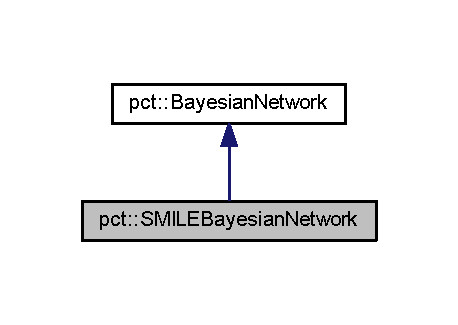
\includegraphics[width=220pt]{classpct_1_1_s_m_i_l_e_bayesian_network__inherit__graph}
\end{center}
\end{figure}


Collaboration diagram for pct\-:\-:S\-M\-I\-L\-E\-Bayesian\-Network\-:\nopagebreak
\begin{figure}[H]
\begin{center}
\leavevmode
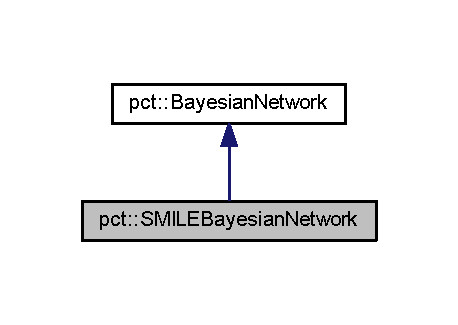
\includegraphics[width=220pt]{classpct_1_1_s_m_i_l_e_bayesian_network__coll__graph}
\end{center}
\end{figure}
\subsection*{Public Member Functions}
\begin{DoxyCompactItemize}
\item 
\hypertarget{classpct_1_1_s_m_i_l_e_bayesian_network_a25dd02f46bca3c668328bc82e9b28c29}{{\bfseries S\-M\-I\-L\-E\-Bayesian\-Network} (D\-S\-L\-\_\-network network)}\label{classpct_1_1_s_m_i_l_e_bayesian_network_a25dd02f46bca3c668328bc82e9b28c29}

\item 
\hypertarget{classpct_1_1_s_m_i_l_e_bayesian_network_aacc0635e0edf94c0dc5d2b6072d409fc}{virtual void {\bfseries add\-Node} (string name, vector$<$ string $>$ values)}\label{classpct_1_1_s_m_i_l_e_bayesian_network_aacc0635e0edf94c0dc5d2b6072d409fc}

\item 
\hypertarget{classpct_1_1_s_m_i_l_e_bayesian_network_a0c1f64f9bcc881cc2d7f0fdeeef68c06}{virtual void {\bfseries add\-Dependency} (string from, string to)}\label{classpct_1_1_s_m_i_l_e_bayesian_network_a0c1f64f9bcc881cc2d7f0fdeeef68c06}

\item 
\hypertarget{classpct_1_1_s_m_i_l_e_bayesian_network_a11ed702c942d6f2f81c3cdbb488b8341}{virtual void {\bfseries write\-File} (string name, File\-Format format)}\label{classpct_1_1_s_m_i_l_e_bayesian_network_a11ed702c942d6f2f81c3cdbb488b8341}

\item 
\hypertarget{classpct_1_1_s_m_i_l_e_bayesian_network_a9d9f695b9d62bff0348f28a84d58ee17}{virtual void {\bfseries set\-Algorithm} (string name)}\label{classpct_1_1_s_m_i_l_e_bayesian_network_a9d9f695b9d62bff0348f28a84d58ee17}

\item 
\hypertarget{classpct_1_1_s_m_i_l_e_bayesian_network_a20b8c919d3ef1e0ec9a93fba9c75e8d7}{virtual void {\bfseries update} ()}\label{classpct_1_1_s_m_i_l_e_bayesian_network_a20b8c919d3ef1e0ec9a93fba9c75e8d7}

\item 
\hypertarget{classpct_1_1_s_m_i_l_e_bayesian_network_af253de2afac4c80467f191dfdb344811}{virtual void {\bfseries calculate\-Distribution} (\hyperlink{classpct_1_1_query}{Query} query)}\label{classpct_1_1_s_m_i_l_e_bayesian_network_af253de2afac4c80467f191dfdb344811}

\end{DoxyCompactItemize}
\subsection*{Additional Inherited Members}


The documentation for this class was generated from the following files\-:\begin{DoxyCompactItemize}
\item 
\hyperlink{network_8hpp}{network.\-hpp}\item 
network.\-cpp\end{DoxyCompactItemize}

\hypertarget{class_test}{\section{Test Class Reference}
\label{class_test}\index{Test@{Test}}
}
\subsection*{Public Member Functions}
\begin{DoxyCompactItemize}
\item 
\hypertarget{class_test_a50697b06fcd7021c126a5bceceb6757c}{void {\bfseries run\-Tests} ()}\label{class_test_a50697b06fcd7021c126a5bceceb6757c}

\end{DoxyCompactItemize}


The documentation for this class was generated from the following files\-:\begin{DoxyCompactItemize}
\item 
test.\-hpp\item 
test.\-cpp\end{DoxyCompactItemize}

\hypertarget{classpct_1_1_token}{\section{pct\-:\-:Token Class Reference}
\label{classpct_1_1_token}\index{pct\-::\-Token@{pct\-::\-Token}}
}


Collaboration diagram for pct\-:\-:Token\-:
\nopagebreak
\begin{figure}[H]
\begin{center}
\leavevmode
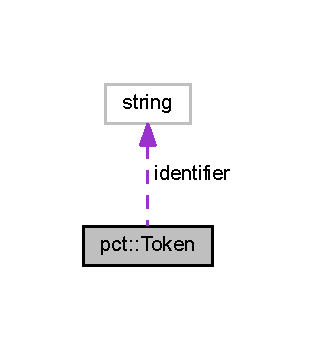
\includegraphics[width=151pt]{classpct_1_1_token__coll__graph}
\end{center}
\end{figure}
\subsection*{Public Types}
\begin{DoxyCompactItemize}
\item 
enum {\bfseries Type} \{ \\*
{\bfseries Left\-Bracket}, 
{\bfseries Right\-Bracket}, 
{\bfseries Equals}, 
{\bfseries Comma}, 
\\*
{\bfseries Pipe}, 
{\bfseries Name}, 
{\bfseries E\-O\-L}
 \}
\end{DoxyCompactItemize}
\subsection*{Public Member Functions}
\begin{DoxyCompactItemize}
\item 
\hypertarget{classpct_1_1_token_a1e704c3bde9b1e03aa06e4e0cd24b9f9}{{\bfseries Token} (Type t)}\label{classpct_1_1_token_a1e704c3bde9b1e03aa06e4e0cd24b9f9}

\item 
\hypertarget{classpct_1_1_token_a2eb1ffd34fa3174c5698269d3603d7c8}{{\bfseries Token} (Type t, string id)}\label{classpct_1_1_token_a2eb1ffd34fa3174c5698269d3603d7c8}

\end{DoxyCompactItemize}
\subsection*{Public Attributes}
\begin{DoxyCompactItemize}
\item 
\hypertarget{classpct_1_1_token_aa086c13ddb36a435dc42d1ff26e00418}{Type {\bfseries type}}\label{classpct_1_1_token_aa086c13ddb36a435dc42d1ff26e00418}

\item 
\hypertarget{classpct_1_1_token_ac3c3a9415583f87fde446ca1342fd77e}{string {\bfseries identifier}}\label{classpct_1_1_token_ac3c3a9415583f87fde446ca1342fd77e}

\end{DoxyCompactItemize}


The documentation for this class was generated from the following file\-:\begin{DoxyCompactItemize}
\item 
token.\-hpp\end{DoxyCompactItemize}

\hypertarget{classpct_1_1_tool}{\section{pct\-:\-:Tool Class Reference}
\label{classpct_1_1_tool}\index{pct\-::\-Tool@{pct\-::\-Tool}}
}


Inheritance diagram for pct\-:\-:Tool\-:\nopagebreak
\begin{figure}[H]
\begin{center}
\leavevmode
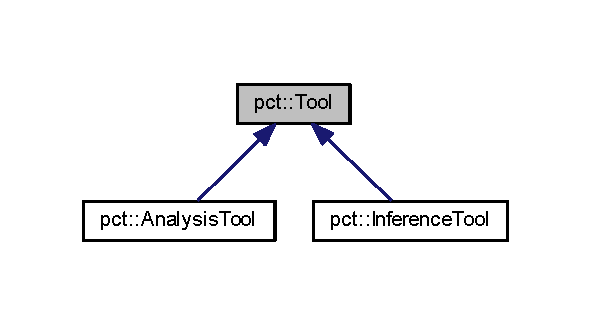
\includegraphics[width=283pt]{classpct_1_1_tool__inherit__graph}
\end{center}
\end{figure}


Collaboration diagram for pct\-:\-:Tool\-:\nopagebreak
\begin{figure}[H]
\begin{center}
\leavevmode
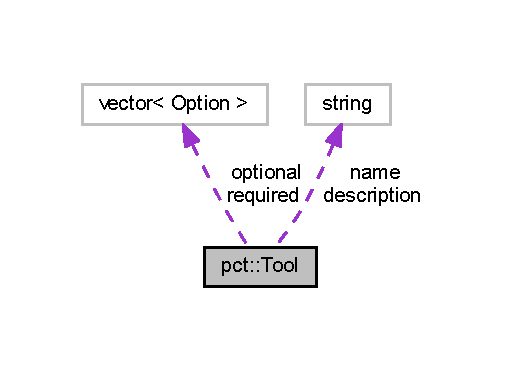
\includegraphics[width=243pt]{classpct_1_1_tool__coll__graph}
\end{center}
\end{figure}
\subsection*{Public Member Functions}
\begin{DoxyCompactItemize}
\item 
\hypertarget{classpct_1_1_tool_a90adc8a035ba612fa866f7fa9599091e}{virtual \hyperlink{classpct_1_1_info_set}{Info\-Set} {\bfseries run} (\hyperlink{classpct_1_1_info_set}{Info\-Set} options)=0}\label{classpct_1_1_tool_a90adc8a035ba612fa866f7fa9599091e}

\item 
\hypertarget{classpct_1_1_tool_a292c57bb278c6cb396e0b98fdb430da6}{string {\bfseries get\-Name} ()}\label{classpct_1_1_tool_a292c57bb278c6cb396e0b98fdb430da6}

\item 
\hypertarget{classpct_1_1_tool_a08c4e95312d0b982ef08423a161435bf}{string {\bfseries get\-Description} ()}\label{classpct_1_1_tool_a08c4e95312d0b982ef08423a161435bf}

\item 
\hypertarget{classpct_1_1_tool_aa0d906602390db5ee0a734e38a076319}{string {\bfseries get\-Usage} ()}\label{classpct_1_1_tool_aa0d906602390db5ee0a734e38a076319}

\item 
\hypertarget{classpct_1_1_tool_ab440971d238b60c0afd84722fa748489}{void {\bfseries incorrect\-Usage} ()}\label{classpct_1_1_tool_ab440971d238b60c0afd84722fa748489}

\item 
\hypertarget{classpct_1_1_tool_ab5f2fddae73cd3466b6230ef78074666}{virtual string {\bfseries get\-Option\-Help} (string name)=0}\label{classpct_1_1_tool_ab5f2fddae73cd3466b6230ef78074666}

\end{DoxyCompactItemize}
\subsection*{Protected Member Functions}
\begin{DoxyCompactItemize}
\item 
\hypertarget{classpct_1_1_tool_a4be774ffb66509ce3324fd067a0141a6}{bool {\bfseries check\-Options} (\hyperlink{classpct_1_1_info_set}{Info\-Set} options)}\label{classpct_1_1_tool_a4be774ffb66509ce3324fd067a0141a6}

\item 
\hypertarget{classpct_1_1_tool_a191caafe159a31f7decb46cbe3f2fe3f}{void {\bfseries display} (string msg, bool verbose)}\label{classpct_1_1_tool_a191caafe159a31f7decb46cbe3f2fe3f}

\item 
\hypertarget{classpct_1_1_tool_a079e22dd0beb78aeb831ebd6622d5e83}{void \hyperlink{classpct_1_1_tool_a079e22dd0beb78aeb831ebd6622d5e83}{output\-Result} (string file, string result)}\label{classpct_1_1_tool_a079e22dd0beb78aeb831ebd6622d5e83}

\begin{DoxyCompactList}\small\item\em Writes a result to the specified file. \end{DoxyCompactList}\end{DoxyCompactItemize}
\subsection*{Protected Attributes}
\begin{DoxyCompactItemize}
\item 
\hypertarget{classpct_1_1_tool_ad34b25a892c0692fdfb78c5321099c00}{string {\bfseries name}}\label{classpct_1_1_tool_ad34b25a892c0692fdfb78c5321099c00}

\item 
\hypertarget{classpct_1_1_tool_aecbec496ecac64124b3d0c8c40ae67ed}{string {\bfseries description}}\label{classpct_1_1_tool_aecbec496ecac64124b3d0c8c40ae67ed}

\item 
\hypertarget{classpct_1_1_tool_a240637721a7943cebd3feb2af447697e}{Option\-List {\bfseries required}}\label{classpct_1_1_tool_a240637721a7943cebd3feb2af447697e}

\item 
\hypertarget{classpct_1_1_tool_a4f59ff09a9258a744f1bbabd5e98835e}{Option\-List {\bfseries optional}}\label{classpct_1_1_tool_a4f59ff09a9258a744f1bbabd5e98835e}

\end{DoxyCompactItemize}


The documentation for this class was generated from the following files\-:\begin{DoxyCompactItemize}
\item 
tool.\-hpp\item 
tool.\-cpp\end{DoxyCompactItemize}

\hypertarget{classpct_1_1_variable}{\section{pct\-:\-:Variable Class Reference}
\label{classpct_1_1_variable}\index{pct\-::\-Variable@{pct\-::\-Variable}}
}


Collaboration diagram for pct\-:\-:Variable\-:\nopagebreak
\begin{figure}[H]
\begin{center}
\leavevmode
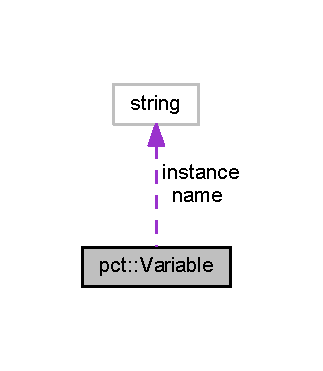
\includegraphics[width=155pt]{classpct_1_1_variable__coll__graph}
\end{center}
\end{figure}
\subsection*{Public Member Functions}
\begin{DoxyCompactItemize}
\item 
\hypertarget{classpct_1_1_variable_afc1e4759b2c0b38129b0b3830b6f6842}{{\bfseries Variable} (string name\-\_\-)}\label{classpct_1_1_variable_afc1e4759b2c0b38129b0b3830b6f6842}

\item 
\hypertarget{classpct_1_1_variable_aff094da93ed282620985ef59af4a834a}{{\bfseries Variable} (string name\-\_\-, string instance\-\_\-)}\label{classpct_1_1_variable_aff094da93ed282620985ef59af4a834a}

\end{DoxyCompactItemize}
\subsection*{Public Attributes}
\begin{DoxyCompactItemize}
\item 
\hypertarget{classpct_1_1_variable_aa8b7c67527f09244e621002317b67ac6}{string {\bfseries name}}\label{classpct_1_1_variable_aa8b7c67527f09244e621002317b67ac6}

\item 
\hypertarget{classpct_1_1_variable_a2193bea3a0433c6fdcf0be593388edc1}{bool {\bfseries instantiated}}\label{classpct_1_1_variable_a2193bea3a0433c6fdcf0be593388edc1}

\item 
\hypertarget{classpct_1_1_variable_ac0d995115059874a355e08020fd8d65f}{string {\bfseries instance}}\label{classpct_1_1_variable_ac0d995115059874a355e08020fd8d65f}

\end{DoxyCompactItemize}


The documentation for this class was generated from the following file\-:\begin{DoxyCompactItemize}
\item 
variable.\-hpp\end{DoxyCompactItemize}

\chapter{File Documentation}
\hypertarget{network_8hpp}{\section{network.\-hpp File Reference}
\label{network_8hpp}\index{network.\-hpp@{network.\-hpp}}
}
{\ttfamily \#include $<$map$>$}\\*
{\ttfamily \#include \char`\"{}smile.\-h\char`\"{}}\\*
{\ttfamily \#include \char`\"{}util\textbackslash{}parser.\-hpp\char`\"{}}\\*
Include dependency graph for network.\-hpp\-:
\nopagebreak
\begin{figure}[H]
\begin{center}
\leavevmode
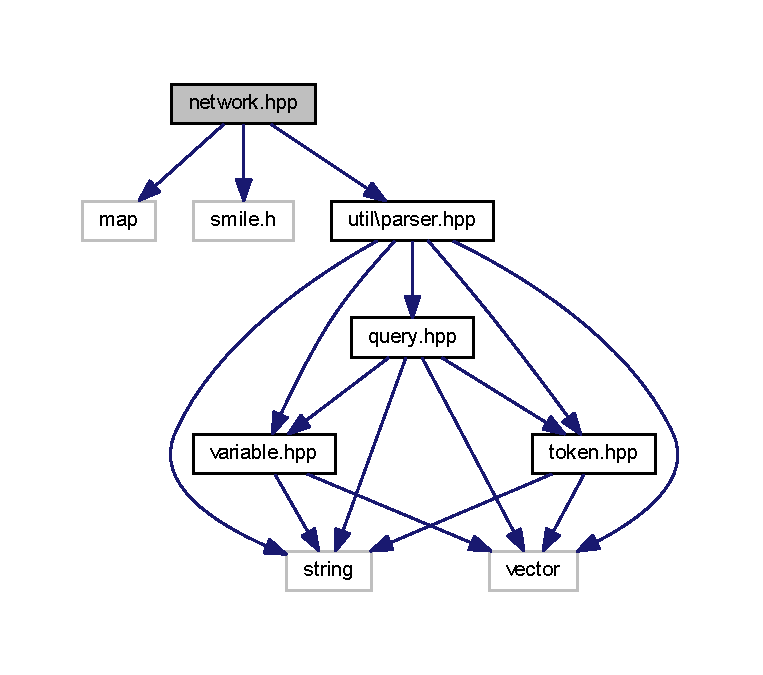
\includegraphics[width=350pt]{network_8hpp__incl}
\end{center}
\end{figure}
This graph shows which files directly or indirectly include this file\-:\nopagebreak
\begin{figure}[H]
\begin{center}
\leavevmode
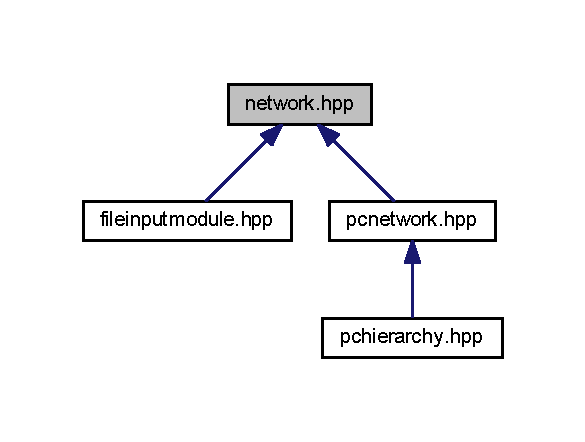
\includegraphics[width=281pt]{network_8hpp__dep__incl}
\end{center}
\end{figure}
\subsection*{Classes}
\begin{DoxyCompactItemize}
\item 
class \hyperlink{classpct_1_1_bayesian_network}{pct\-::\-Bayesian\-Network}
\item 
class \hyperlink{classpct_1_1_s_m_i_l_e_bayesian_network}{pct\-::\-S\-M\-I\-L\-E\-Bayesian\-Network}
\end{DoxyCompactItemize}
\subsection*{Enumerations}
\begin{DoxyCompactItemize}
\item 
enum {\bfseries File\-Format} \{ {\bfseries D\-S\-L}, 
{\bfseries T\-X\-T}
 \}
\end{DoxyCompactItemize}

\hypertarget{pct_8hpp}{\section{pct.\-hpp File Reference}
\label{pct_8hpp}\index{pct.\-hpp@{pct.\-hpp}}
}
{\ttfamily \#include $<$string$>$}\\*
{\ttfamily \#include \char`\"{}infoset.\-hpp\char`\"{}}\\*
{\ttfamily \#include \char`\"{}tools/tool.\-hpp\char`\"{}}\\*
Include dependency graph for pct.\-hpp\-:\nopagebreak
\begin{figure}[H]
\begin{center}
\leavevmode
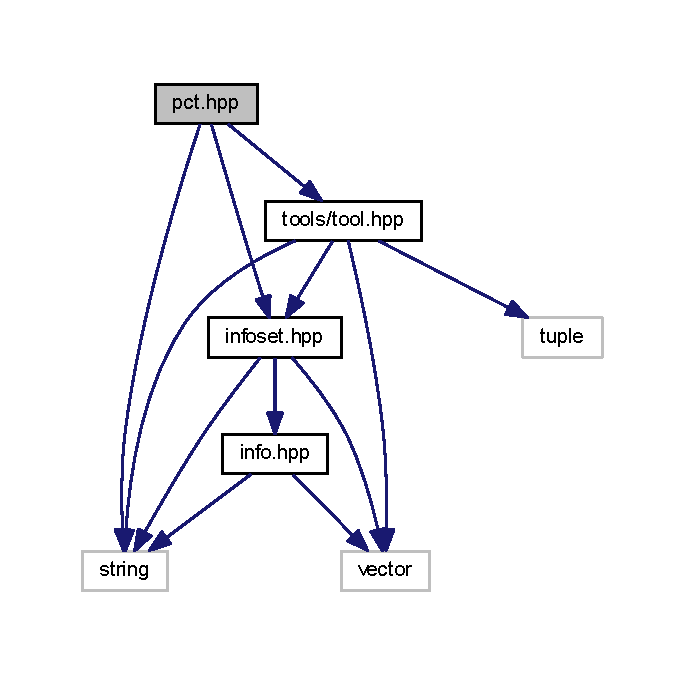
\includegraphics[width=329pt]{pct_8hpp__incl}
\end{center}
\end{figure}
\subsection*{Classes}
\begin{DoxyCompactItemize}
\item 
class \hyperlink{classpct_1_1_predictive_coding_toolbox}{pct\-::\-Predictive\-Coding\-Toolbox}
\begin{DoxyCompactList}\small\item\em Main class for the Predictive Coding Toolbox. \end{DoxyCompactList}\end{DoxyCompactItemize}

%--- End generated contents ---

% Index
\newpage
\phantomsection
\addcontentsline{toc}{part}{Index}
\printindex

\end{document}
